\clearpage\section{Технологическая часть}
\subsection{Средства реализации}
Реализации написаны на языке Си (C), стандарт 2011 года (C11). Для потоков, мьютекса и условных переменных применяется интерфейс потоков POSIX в реализации winpthreads, поставляемой с MSYS2. Использован компилятор GCC 14.2.0, среда UCRT64. Измерительная сборка выполняется с параметрами \texttt{-std=c11 -O0 -Wall -Wextra -Wpedantic -pthread}, без отладочной информации и без оптимизации.

Счётчики гистограммы имеют тип беззнакового 64-разрядного целого числа. Размер изображения ограничен условием $N\le\lfloor(2^{64}-1)/255\rfloor$ и доступной памятью. Это исключает переполнение суммы яркостей. Критерий Оцу вычисляется с использованием вещественного типа расширенной точности \texttt{long double}; поэтому для практически равных максимумов на иных больших входах округление может влиять на выбранный порог. В функциональных проверках совпадение с точным эталоном подтверждено. Между последовательной и параллельной версиями порядок вычисления критерия одинаков.

Исходные тексты разделены на модули сегментации, обработки изображений и командного интерфейса. Основные функции подключены непосредственно из исходных файлов в приложении~А. Один локальный массив гистограммы занимает 2048 байт, $q$ таких массивов --- $2048\cdot q$ байт. Дополнительно выделяются описатели потоков и структуры синхронизации; память стеков управляется библиотекой потоков и операционной системой.

\subsection{Пример сегментации}
На рисунке~\ref{fig:example} представлены сгенерированный полутоновый фантом и его бинарная маска. Фантом составлен из эллиптических областей двух диапазонов яркости с псевдослучайным шумом; он служит воспроизводимым учебным входом и не является рентгеновским снимком пациента. Для размера $512\times512$ получен порог $T=64$. Последовательная и параллельная маски совпали.
\begin{figure}[H]\centering
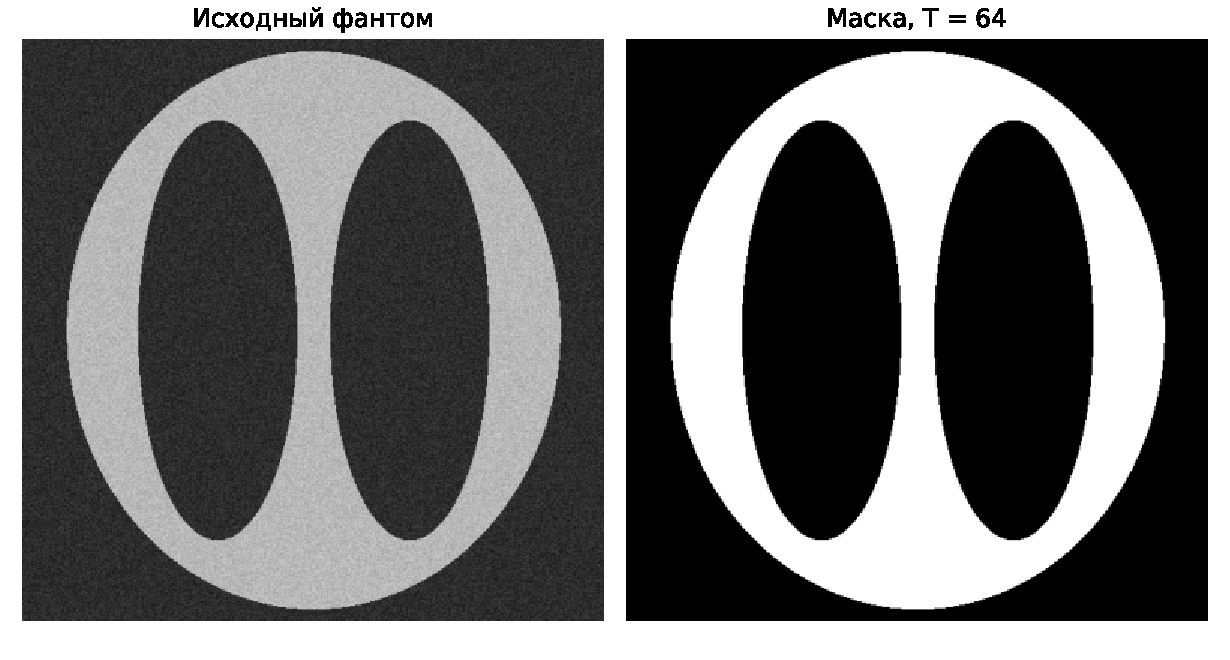
\includegraphics[width=\textwidth]{figures/example.pdf}
\caption{Исходный синтетический фантом и результат сегментации}\label{fig:example}
\end{figure}
